\usepackage{tikz}
\PassOptionsToPackage{hyphens}{url}\usepackage{hyperref}
\usepackage{tcolorbox}
\usepackage{listingsutf8}
\tcbuselibrary{listingsutf8}
\tcbuselibrary{skins}
\usepackage{menukeys}
\usepackage{lmodern}
\usepackage{fontawesome}
\usepackage{qrcode}

%Graphics path
\graphicspath{{./images/}}


%Defined colors
\definecolor{mushroom}{HTML}{FEF2E4}
\definecolor{onion}{HTML}{FD974F}
\definecolor{redpepper}{HTML}{C60000}
\definecolor{driftwood}{HTML}{805A3B}
\definecolor{salmon}{HTML}{F56C57}
\definecolor{caviar}{HTML}{F77604}
\definecolor{lettuce}{HTML}{B8D20B}
\definecolor{blackseaweed}{HTML}{231B12}



%Selected fonts
\newcommand{\fontpag}{\fontfamily{pag}\selectfont}
\newcommand{\fontppl}{\fontfamily{ppl}\selectfont}
\newcommand{\fontqag}{\fontfamily{qag}\selectfont}
\newcommand{\fontcode}{\fontfamily{phv}\selectfont}



\newcommand*{\heading}[1]{{\fontpag\Huge\uppercase{\textbf{#1}}}\\}


%Decorated texts
\newcommand*{\blacktextbox}[1]{\fontpag\Huge\textbf{\fcolorbox{black}{black}{\color{white}\uppercase{#1}}}}



%Formatted texts

%-- Shell console input
\newcommand*{\shi}[1]{\textcolor{yellow!50}{\ttfamily\bfseries \$\quad}\textcolor{mushroom}{\ttfamily #1
%{\tikz[baseline]{\draw node [opacity=0.25, anchor=base] {{{\return}}};}}
}}

%-- Python console output
\newcommand*{\pyi}[1]{\textcolor{yellow!50}{\ttfamily\bfseries >>>\quad}\textcolor{white}{\ttfamily #1
%{\tikz[baseline]{\draw node [opacity=0.25, anchor=base] {{{\return}}};}}
}}


%-- Console output (multiline)
\lstnewenvironment{sho}{
\lstset{
basicstyle=\color{caviar}\small\ttfamily
}}{}

%-- Shell console input/output
\newcommand{\shio}[2]{%
\shi{#1}\\{\color{caviar}\small\detokenize{#2}}\\
}

%-- Python console input/output
\newcommand{\pyio}[2]{%
\pyi{{#1}}\\{\ttfamily\color{caviar}\small#2}\\
}


%Defined objects

%-- Terminal box environment
\newtcolorbox{terminal}{
title={\foreach \x in {red!80, yellow!80, green!90}{\tikz{\draw[\x, fill=\x] circle (4pt);}\;}}\hspace{60mm}{\color{blackseaweed}Shell},
before skip=6mm,
width=12cm,
height=8cm,
rightrule=0mm,
leftrule=0mm,
bottomrule=0mm,
toptitle=1mm,
bottomtitle=1mm,
colframe=gray!70,
colback=black!70,
colupper=mushroom}

%-- Python code environment
\newenvironment{pycode}[1]{\tcblisting{
title={\foreach \x in {red!80, yellow!80, green!90}{\tikz{\draw[\x, fill=\x] circle (4pt);}\;}}\hspace{5.2cm}\faFileTextO\;{#1},
fonttitle=\color{black}\small,
before skip=6mm,
width=12cm,
height=9cm,
rightrule=0mm,
leftrule=0mm,
bottomrule=0mm,
toptitle=1mm,
bottomtitle=1mm,
colframe=gray!70,
colback=gray!3,
colupper=blackseaweed,
left=20pt,
listing only,
listing options={
language=Python,
numbers=left,
numberstyle=\color{black}\scriptsize,
numbersep=10pt,
tabsize=4,
showstringspaces=false,
basicstyle=\color{blackseaweed}\fontcode\small,
keywordstyle=\color{blue!80}\fontcode\bfseries,
stringstyle=\color{salmon}\fontcode,
commentstyle=\color{gray!90}\fontcode
}}
}{%
\endtcblisting
\tikz[overlay, remember picture]{
%\draw[blue] (0,0) grid (5,5);
\draw[black!20,fill=black!30,opacity=0.25] (0,0) rectangle (0.75,8.675);
}}

%-- Overlay object
\newcommand{\overlayat}[2]{\tikz[overlay, remember picture]{\node at #1 {#2};}}

%Beamer config.

%-- Cover
\newcommand{\coverframe}[2]{%
\begin{frame}
\begin{columns}
\begin{column}{0.4\textwidth}
\tikz[remember picture, overlay]{
\node at (2.2,-0.2) {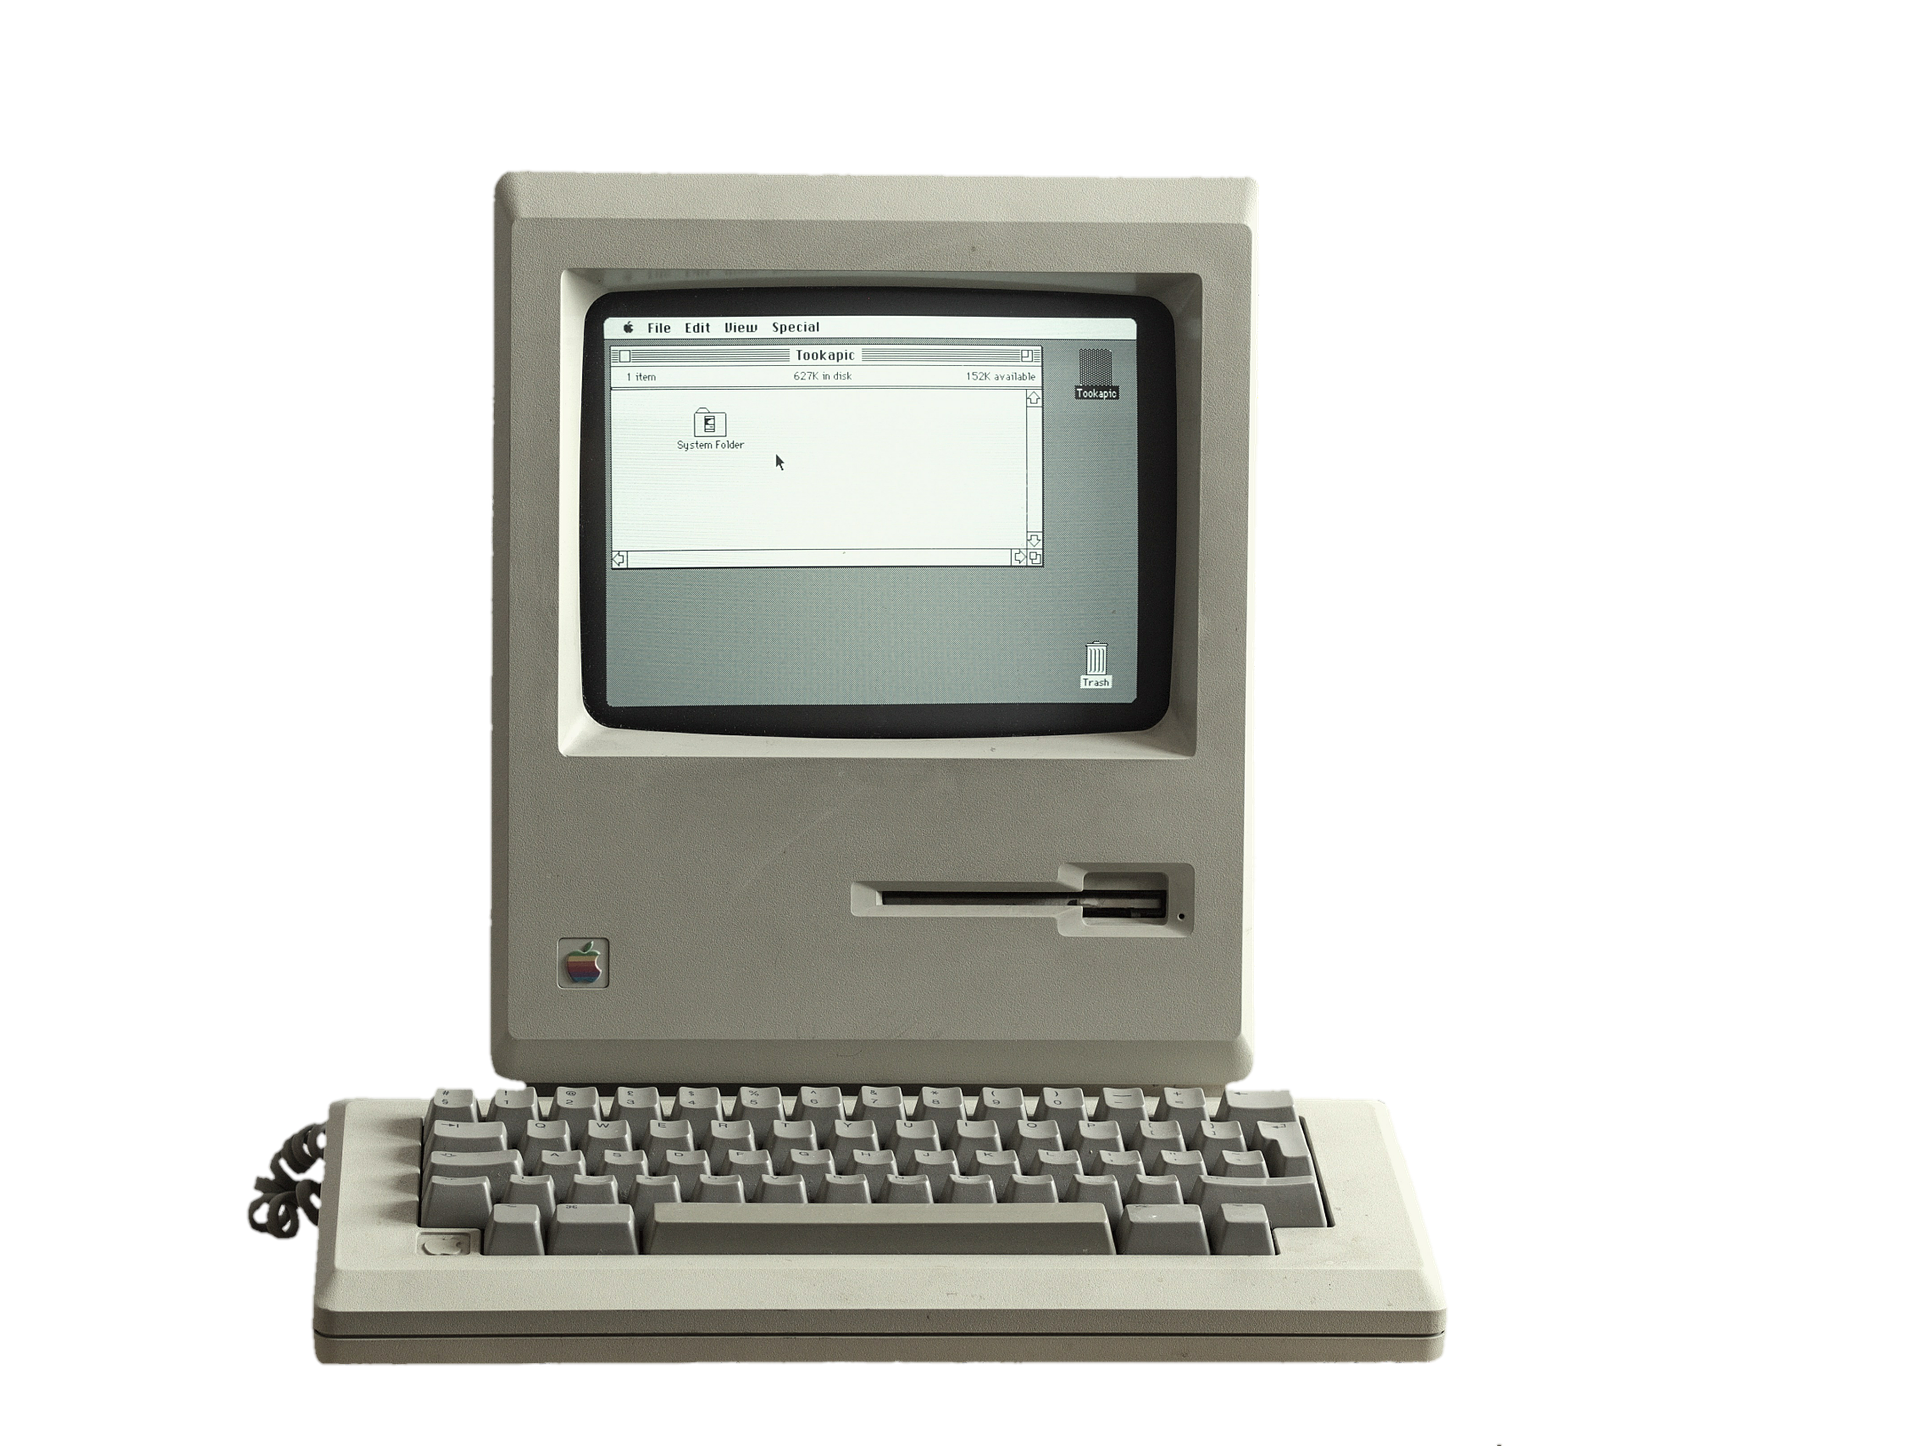
\includegraphics[scale=0.25]{apple_ii}};
}
\end{column}
\begin{column}{0.6\textwidth}
 \begin{center}
    {\fontqag\tiny\uppercase{\textbf{From Zero to Hero}}}\\
    {\fontqag\color{onion}\large\uppercase{Python the Hardway}}
    \vspace{5mm}\\
    {\fontpag\large{\faStar\,\faStar\,\faStar\,\faStar\,\faStar}}
    \vspace{3mm}\\
    \heading{#2}
    {\fontqag\scriptsize\uppercase{-R.Promkam-}}
    \vspace{10mm}\\
    {\fontpag\tiny\uppercase{powerful programming language}}
    \vspace{1mm}\\
    {\fontpag\Huge\textbf{\fcolorbox{black}{black}{\color{white}\uppercase{EPISODE}}\fbox{\uppercase{\;#1\;}}}}   
 \end{center}   
 \vspace{10mm}
 \hfill
\includegraphics[scale=0.03]{python_logo}
\end{column} 
\end{columns}
\end{frame}
}

%-- End slide
\newcommand*{\episodeisdone}{
\usebackgroundtemplate{}
\begin{frame}
\tikz[overlay]{%
\fill[blackseaweed] (-1,5) rectangle (13,-8);
}
\begin{center}

\includegraphics[scale=0.3]{python_logo} 
\end{center}
\end{frame}
}


%-- Frame title
\newcommand*{\ftitle}[1]{\frametitle{\color{salmon}\fontpag\huge\uppercase{\textbf{#1}}}}

%-- Horizontal Beamer BG
\newcommand*{\hbg}{\usebackgroundtemplate{
\tikz[overlay]{
\draw[fill=blackseaweed,blackseaweed] (0,0) rectangle (13,-3.5);
\node at (12,-1.8) {
\includegraphics[scale=0.22]{python_logo}};
%\draw[fill=black!80,black!80] (10,-0.8) rectangle (12,-1.2);
%\draw[fill=mushroom,mushroom] (10,-1) circle (18pt);
%\draw[fill=redpepper,redpepper] (12,-1.5) rectangle (12.1,-6);
}}}

%-- Vertical Beamer BG
\newcommand*{\vbg}{
\usebackgroundtemplate{
\tikz[overlay]{
\draw[fill=blackseaweed,blackseaweed] (0,0) rectangle (5,-10);
\draw[fill=mushroom,mushroom] (4.5,-0.65) circle (7pt);
}}}


















